\question 归并排序有两个基本阶段,第一个阶段是( )
\par\twoch{\textcolor{red}{生成初始归并段}}{从归并序列选出最小值(最大值)}{将文件记录读入内存}{进行多遍归并}
\begin{solution}本题考察归并排序处理过程,详见归并排序的知识点
\end{solution}
\question 下列关于外部排序说法正确的是( )
\par\fourch{内存与外设交换信息的时间只是外排序总时间的一小部分}{外部排序就是在外存上进行排序,无需内存参与}{\textcolor{red}{败者树是一棵完全二叉树}}{置换-选择排序得到的初始归并段长度一定相等}
\begin{solution}A:影响外排序时间的主要因素就是内存与外设交换信息的总次数,所以A错误。
B:外部排序也是在内存上进行排序,只不过需要分为多步而已,所以B错误。
C:从败者树的构建方式可知,败者树是一棵完全二叉树,所以C正确。
\end{solution}
\question 一组记录的关键字为{25,50,15,35,80,85,20,40,36,70},其中含有5个长度为2的有序表,用归并排序方法对该序列进行一趟归并后的结果是(
)
\par\fourch{\textcolor{red}{15,25,35,50,20,40,80,85,36,70}}{15,25,35,50,80,20,85,40,70,36}{15,25,50,35,80,85,20,36,40,70}{15,25,35,50,80,20,36,40,70,85}
\begin{solution}根据归并算法的思想,对5个长度为2的有序表一趟归并后得到两个长度为4的有序表和一个长度为2的有序表,只有A满足。
\end{solution}
\question 某个文件经内部排序得到80个初始归并段。如果操作系统要求一个程序同时可用的输入/输出文件的总数不超过15个,则按多路归并至少需要(
)趟可以完成排序
\par\twoch{\textcolor{red}{2}}{3}{4}{5}
\begin{solution}不妨设采用m路归并,则至少需要m个输入缓冲区和1个输出缓冲区。因为一个缓冲区对应一个文件,所以m+1=15,解得m=14,所以可做14路归并。假设需要s趟可以完成排序,则s=
log(1480) =2。
\end{solution}
\question 假设在磁盘上存放有375
000个记录,做5路平衡归并排序,内存工作区能容纳600个记录,为把所有记录都排好序,需要作(
)趟归并排序
\par\twoch{3}{\textcolor{red}{4}}{5}{6}
\begin{solution}假设做m路平衡归并排序,且有n个初始归并段,则归并趟数为
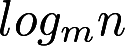
\includegraphics[width=0.45833in,height=0.14583in]{texmath/6261695Cdpi7B3507Dlog_mn}。所以此题只需求出初始归并段n即可,n=375
000/600=625。故归并趟数为 log(5625) =4。
\end{solution}
\question 在外部排序算法中,最佳归并树主要的作用是( )
\par\twoch{产生初始归并段}{完成归并排序}{\textcolor{red}{对归并排序进行优化}}{增大归并路树}
\begin{solution}A:产生初始归并段的工作应该由置换---选择排序完成,故A选项错误。
设输入的关键字满足k1大于k2远远大于kn,缓冲区大小为m,用置换-选择排序方法可产生
n/m 个初始归并段。
B:因为最佳归并树是针对排序之后的初始归并段操作,所以归并排序不可能由最佳归并树完成,故B选项错误。
C:最佳归并树仿造赫夫曼树的构造过程,以初始归并段的长度为权值,构造具有最小带权路径长度的赫夫曼树,可以有效地减少归并过程中的读写记录数,以加快外部排序的速度,故C选项正确。
D:增大归并路数应该是由败者树来完成的,故D选项错误。
\end{solution}
\question 假设有5个初始归并段,每个归并段有20个记录,采用5路平衡归并排序,若采用败者树的方法,总的排序码比较次数不超过(
)
\par\twoch{20}{\textcolor{red}{300}}{396}{500}
\begin{solution}假设采用k路平衡归并排序算法,则败者树的高度为
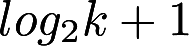
\includegraphics[width=0.67708in,height=0.15625in]{texmath/71308d5Cdpi7B3507Dlog_2k2B1}。且在每次调整后,找下一个具有最小排序码记录时,最多做
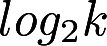
\includegraphics[width=0.39583in,height=0.14583in]{texmath/c7c1e85Cdpi7B3507Dlog_2k}
次排序码比较。由题意可知,总共有100个记录,所以总的比较次数不超过100*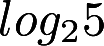
\includegraphics[width=0.38542in,height=0.16667in]{texmath/36a8485Cdpi7B3507Dlog_25}
的向上取整 =300。
注意:采用败者树进行k路平衡归并的外部排序算法,其总的归并效率与k无关。
\end{solution}
